\documentclass{article}
\usepackage[utf8]{inputenc}
\usepackage{amsmath}
\usepackage[spanish]{babel}
\usepackage{graphicx}
\usepackage{float}


\newcommand\tab[1][1cm]{\hspace*{#1}}
\begin{document}



\section*{Problema A}
Nombre: Juan Sebastian Vargas\\
 Codigo: 201215310\\
Fecha: 20/05/16

\section{Algoritmo Solici\'on}
El Algoritmo consta de una lectura de los datos desde $args [i]$ en el método main, y de esta manera se procede a calcular esta ecuación: 
\begin{equation}
    \frac{p}{q}=\frac{\text{trans}\Xi_n+\text{per}}{10^m\Xi_n}
\end{equation}
Donde $\Xi_n $ es una sucesión de $n$ nueves seguidos, por ejemplo, $\Xi_2=99$.
Luego se procede asegurare que estos dos números sean primos relativos mediante el algoritmo Euclidiano. 

\section{Complejidades}
En la lectura de datos no tenemos llamadas repetitivas, ya que solo son necesarias para inicializar el programa. 
Para resolver la ecuación se requiere de un método auxiliar para generar la cadena de 9’s, el cual requiere de n pasadas para lograr esto,(de existir un método en java mas eficiente el calculo cambiaria). \\
Despues se requiere aplicarles el GCD a los números, el cual tiene $ O(N)$ con $N=log(a)+log(b)$.
Su complejidad espacial es de $O(0)$ ya que solo se tienen que guardar 7 datos en cualquier caso


 
\begin{figure}[h]

 \scalebox{0.65}{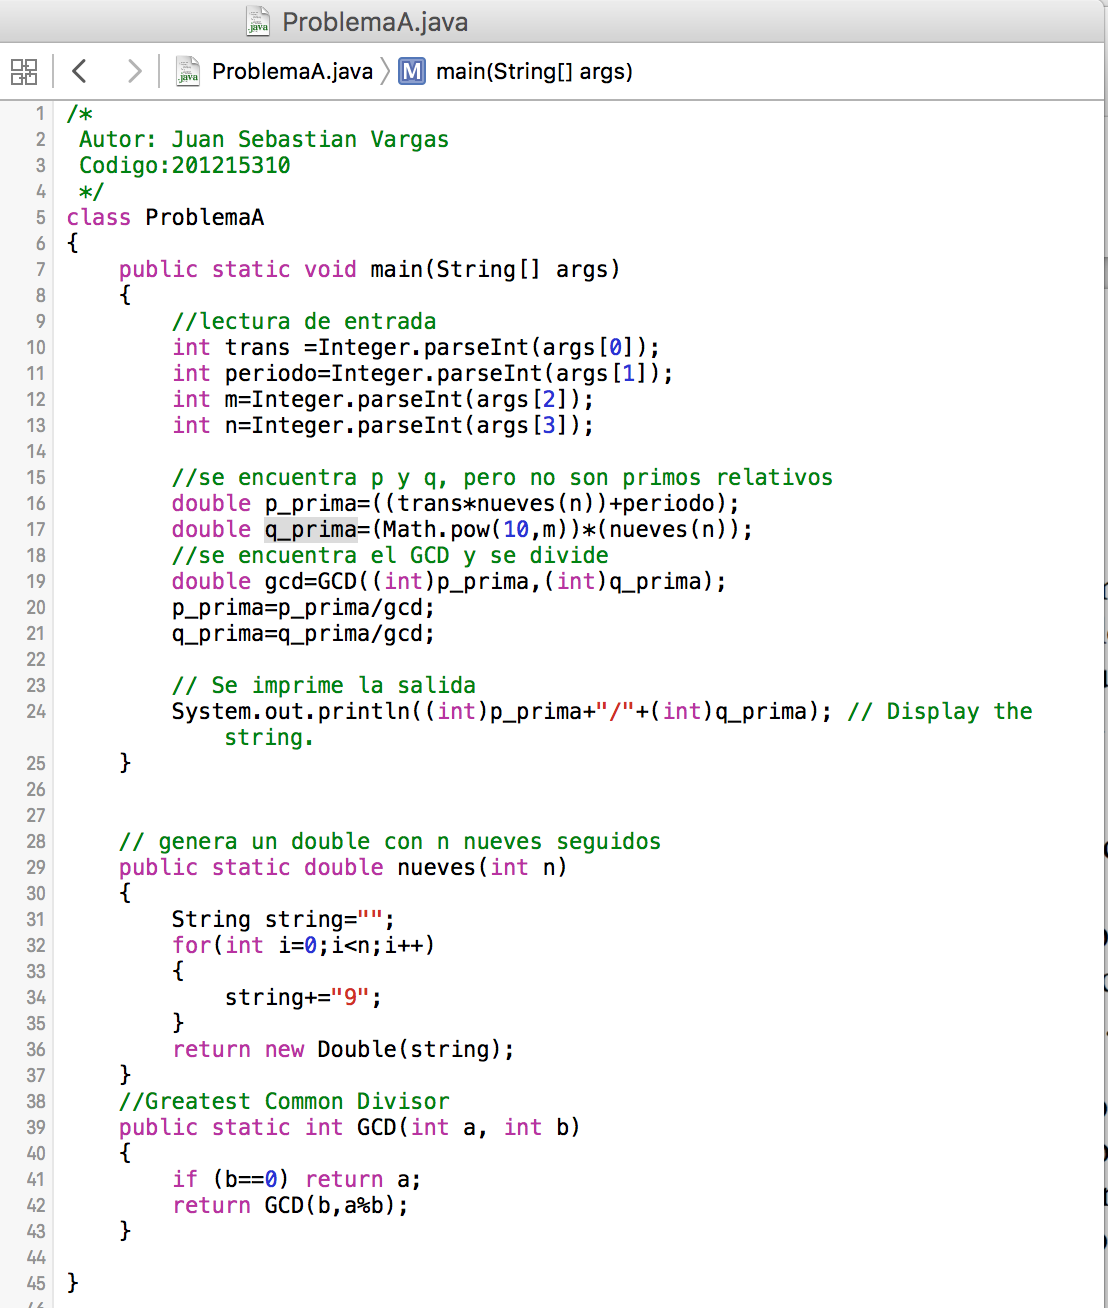
\includegraphics{ProblemaA.png}}
 \caption{Algoritmo}
 \label{Al}
\end{figure}



\end{document}